\documentclass[aspectratio=169]{beamer}

\usepackage[utf8]{inputenc}
\usepackage[T1]{fontenc}

\usepackage{xcolor}
\definecolor{darkgreen}{rgb}{0,0.6,0}
\usepackage[scaled=0.8]{beramono}

% \usepackage[euler-digits]{eulervm}
%\usefonttheme[onlymath]{serif}

\usepackage{listings}
% \usepackage{amsmath}
% \usepackage{amssymb}
% \usepackage{oz}
% \usepackage{mathpartir}
% \usepackage{cancel}
% \usepackage{graphbox}

% \input{macros}
% % \usepackage{../latex/Why3}
% \input{options}
%\newcommand{\why}{\lstinline[language=why3]}


%\setbeamertemplate{navigation symbols}{}%remove navigation symbols
% \setbeamercolor{footline}{fg=blue}
\setbeamerfont{footline}{family=\sffamily}
\setbeamertemplate{navigation symbols}{%
    \usebeamerfont{footline}%
    \usebeamercolor[fg]{footline}%
    \hspace{1em}%
    \insertframenumber/\inserttotalframenumber
}

\usepackage{tikz}
\usetikzlibrary{shapes,arrows,shadows,backgrounds}
\tikzstyle{bloc} = [rectangle, draw, fill=green!30,
     text centered, rounded corners]
\tikzstyle{tool} = [rectangle, draw, fill=red!30,
    text centered]
\tikzstyle{blocl} = [rectangle, draw, color=black!50, fill=green!10,
     text centered, rounded corners]
\tikzstyle{tooll} = [rectangle, draw, color=black!50, fill=red!10,
     text centered]
\tikzstyle{line} = [draw, -triangle 45]
\tikzstyle{linel} = [draw, color=black!50,-triangle 45]
\tikzstyle{elem} = [ellipse, draw, top color=green!5, bottom color=green!30,
     text centered, rounded corners, drop shadow]
\tikzstyle{newtool} = [tool, dashed, top color=blue!10, bottom color=blue!40]
\tikzstyle{newelem} = [elem, dashed, top color=green!10, bottom color=green!40]
\tikzstyle{lib} = [rectangle, draw, top color=yellow!4, bottom color=yellow!30,
    text centered, rounded corners, drop shadow, shading=axis]

\usetikzlibrary{decorations.text}

\setbeamertemplate{blocks}[rounded][shadow=true]
\setbeamercolor{block title}{bg=green!20}
\setbeamercolor{block body}{bg=green!10}
\setbeamercolor{block title alerted}{bg=red!20}
\setbeamercolor{block body alerted}{bg=red!10}
\setbeamercolor{block title example}{bg=blue!20}
\setbeamercolor{block body example}{bg=blue!10}

\usepackage{./why3lang}

%\input{../../../talks/latex/macros-slides-claude}
\lstnewenvironment{whycode}{\lstset{language=why3}}{}
% \lstnewenvironment{whycodesmall}{\lstset{language=why3}\lstset{basicstyle={\ttfamily\footnotesize\color{blue}}}}{}
% \lstnewenvironment{ocamlcode}{\lstset{language={[Objective]Caml}}}{}
% \newcommand{\of}[1]{\lstinline[framesep=0pt]{#1}}
% \lstset{basicstyle={\ttfamily\small}}

% \definecolor{test}{rgb}{.95,.45,.65}
% \definecolor{myblue}{rgb}{0.25,0.41,0.88}

\definecolor{links}{HTML}{2A1B81}
\hypersetup{colorlinks,linkcolor=,urlcolor=links}

\let\oldemph\emph\renewcommand{\emph}[1]{\oldemph{\color{blue} #1}}
\let\oldtexttt\texttt\renewcommand{\texttt}[1]{\oldtexttt{\color{black} #1}}
\newcommand{\m}[1]{\(\color{darkgreen}#1\)}
\newcommand{\mm}[1]{\[\color{darkgreen}#1\]}
\newcommand{\cit}[1]{\hfill{\footnotesize\color{darkgreen}[#1]}}


% \titlegraphic{
%  \includegraphics[width =0.18\textwidth]{../images/logo-why3-hires.png} \hfill
%  \includegraphics[width =0.2\textwidth]{../images/proofinuse.png}}

\title{Experiments with Alt-Ergo 2.6}

\author{Claude~Marché, Matteo~Manighetti}

\date{Decysif/OCamlPro meeting, December 10th, 2024}

\lstset{basicstyle={\ttfamily\footnotesize}}

\begin{document}

\lefthyphenmin=30

\begin{frame}{}
  \maketitle
\end{frame}

\begin{frame}
  \frametitle{Outline}
  \tableofcontents
\end{frame}

  \AtBeginSection[]{
  \begin{frame}
    \frametitle{Outline}
    \tableofcontents[currentsection]
  \end{frame}
}

\section{Alt-Ergo}

\subsection{Counterexamples}

\begin{frame}{Counterexamples}

  \begin{block}{Issues on Alt-Ergo side}
  \begin{itemize}
  \item Syntax \texttt{.k0}, \texttt{.k1} in models: what does it
    mean? Issue reported
    \url{https://github.com/OCamlPro/alt-ergo/issues/1270}
  \item Negative real constants. Issue reported \url{https://github.com/OCamlPro/alt-ergo/issues/1271}
  \end{itemize}
\end{block}
\vfill
\begin{block}{Results from Why3 on Decysif benchmarks}

    To be investigated, so far quite a lot of issues remains on Why3
    side.

  \end{block}
\end{frame}

\begin{frame}{Actions regarding counterexamples}

  What else?
  \begin{itemize}
  \item investigate issues from the Why3 side (all the ``warnings'')
  \item On OCamlPro side?
  \end{itemize}

\end{frame}

\subsection{Bitvectors}

\begin{frame}{Bitvectors}

  \begin{block}{Issues on Alt-Ergo side}
  \begin{itemize}
  \item AE does not support ``overflow'' predicates \texttt{bvuaddo}, \texttt{bvssubo}, etc.

  \item Does not support \texttt{bv2int}, only \texttt{bv2nat}

  \end{itemize}

\end{block}

\vfill

  \begin{block}{Comparison BV vs noBV}

    Next slides

  \end{block}
\end{frame}

\begin{frame}[fragile]{Benchmarking BV support}

  913 VCs from Why3 examples involving bitvectors

%  \begin{scriptsize}
\begin{verbatim}
== Statistics per prover: number of proof attempts, successful ones, time (minimum/maximum/average) in seconds ==
  Alt-Ergo 2.6.0                :   914   555   0.01   4.41   0.13
  Alt-Ergo 2.6.0 (BV)           :   914   583   0.01   4.56   0.11
  CVC5 1.1.2                    :   914   685   0.01   4.76   0.19
  Z3 4.13.2                     :   914   707   0.00   4.28   0.07
\end{verbatim}
  % \end{scriptsize}

  \begin{block}{Good news}
    BV support is better than no support
  \end{block}

\end{frame}

\begin{frame}{AE no BV versus AE BV}

  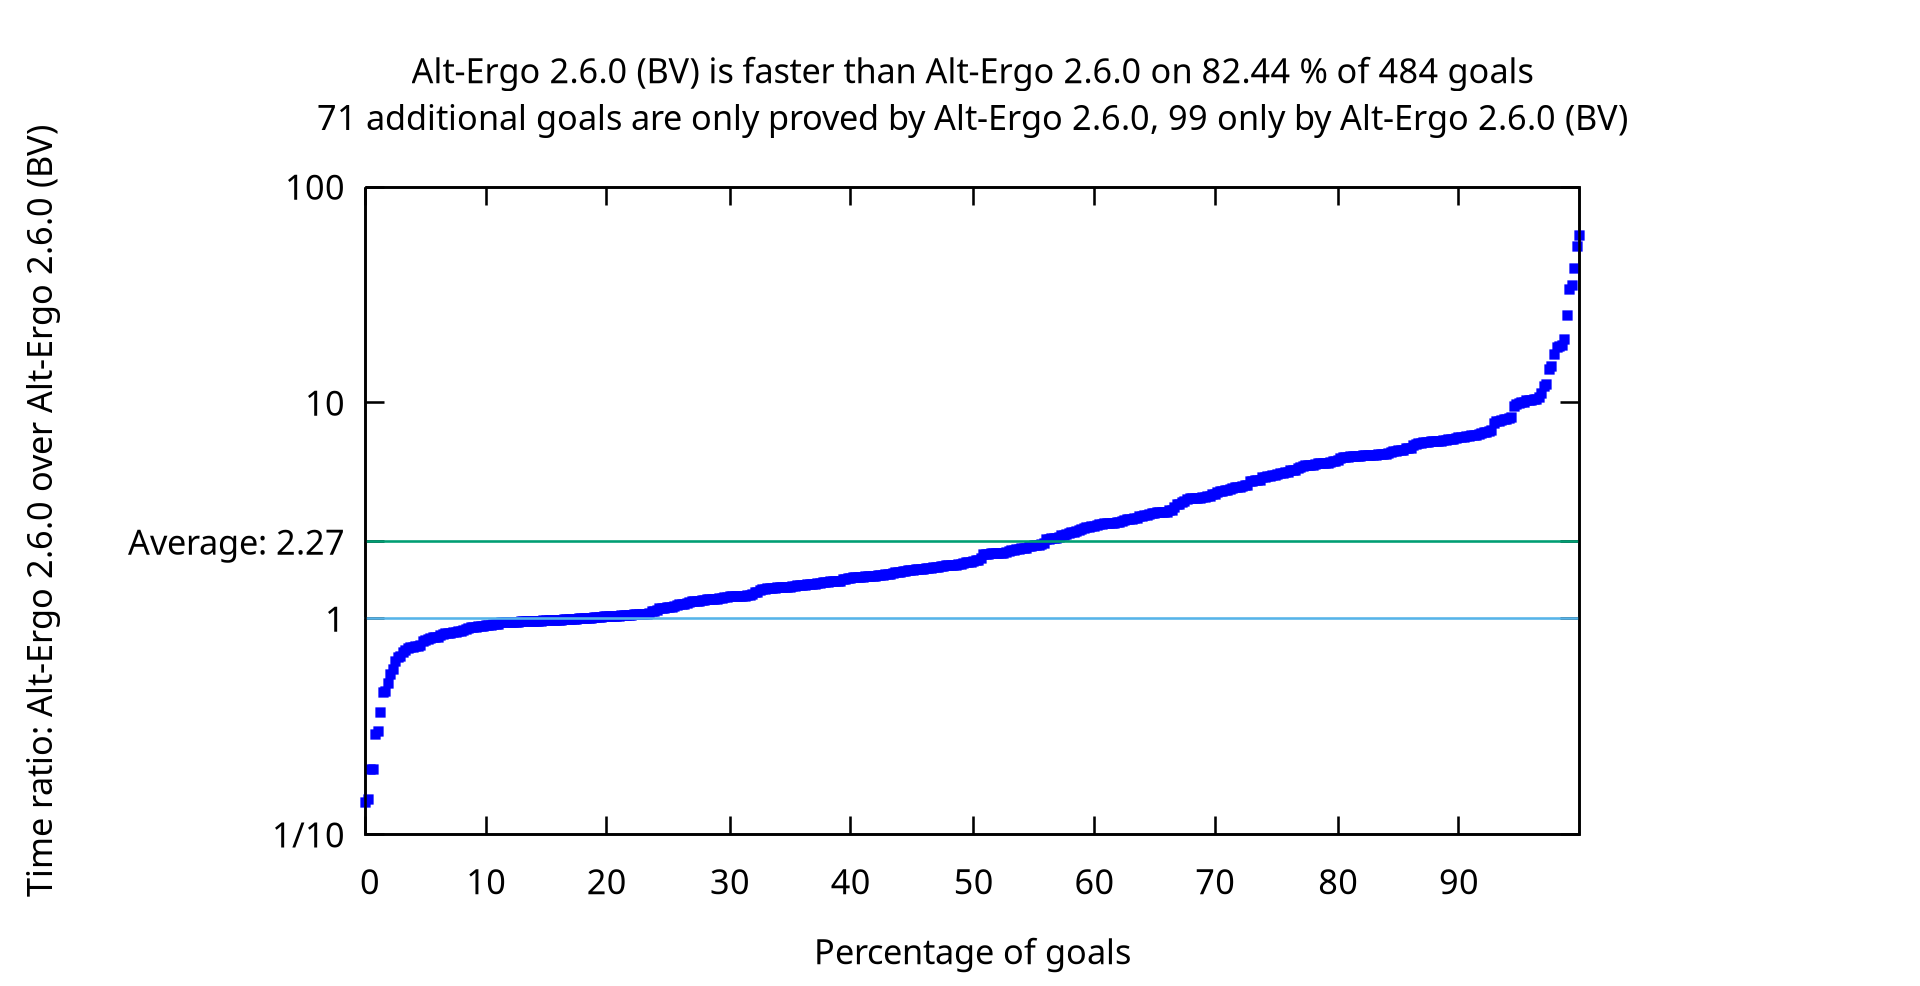
\includegraphics[width=\textwidth]{AEvsAEBV.png}

\end{frame}

\begin{frame}{CVC5 versus AE BV}

  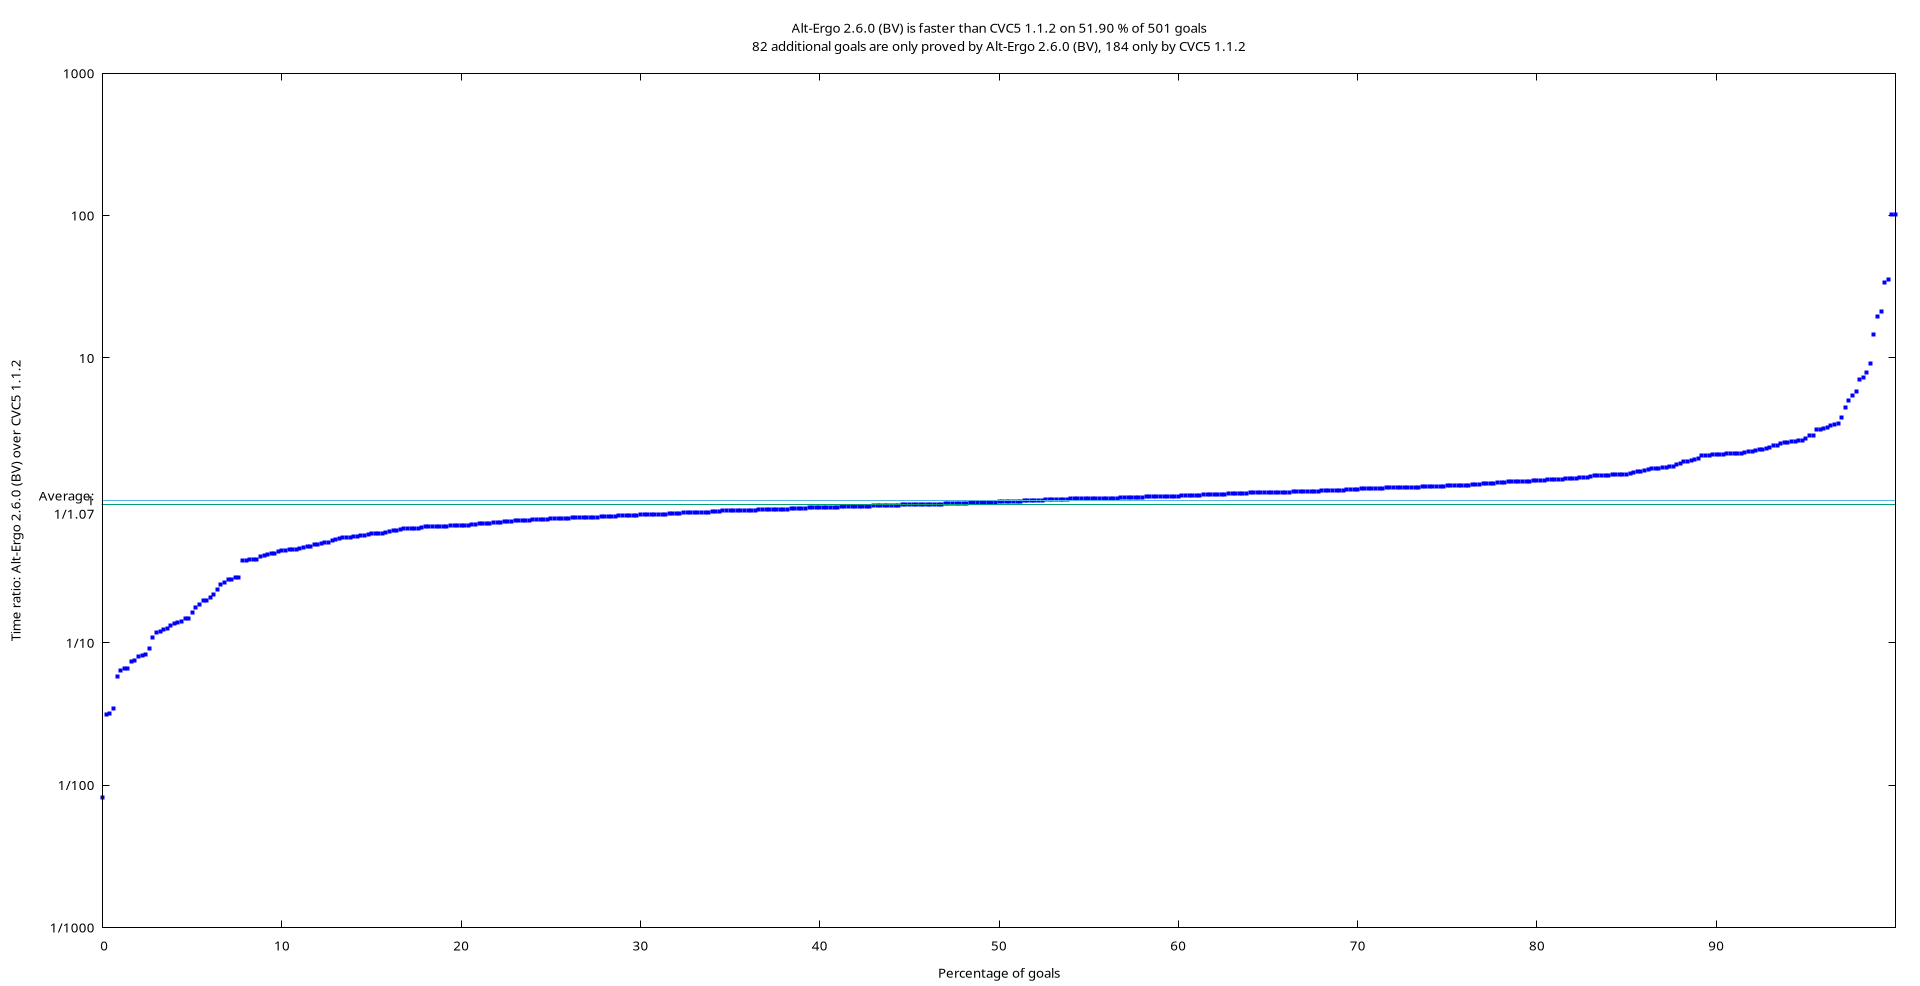
\includegraphics[width=\textwidth]{AEBVvsCVC5.png}

\end{frame}

\begin{frame}{Z3 versus AE BV}

  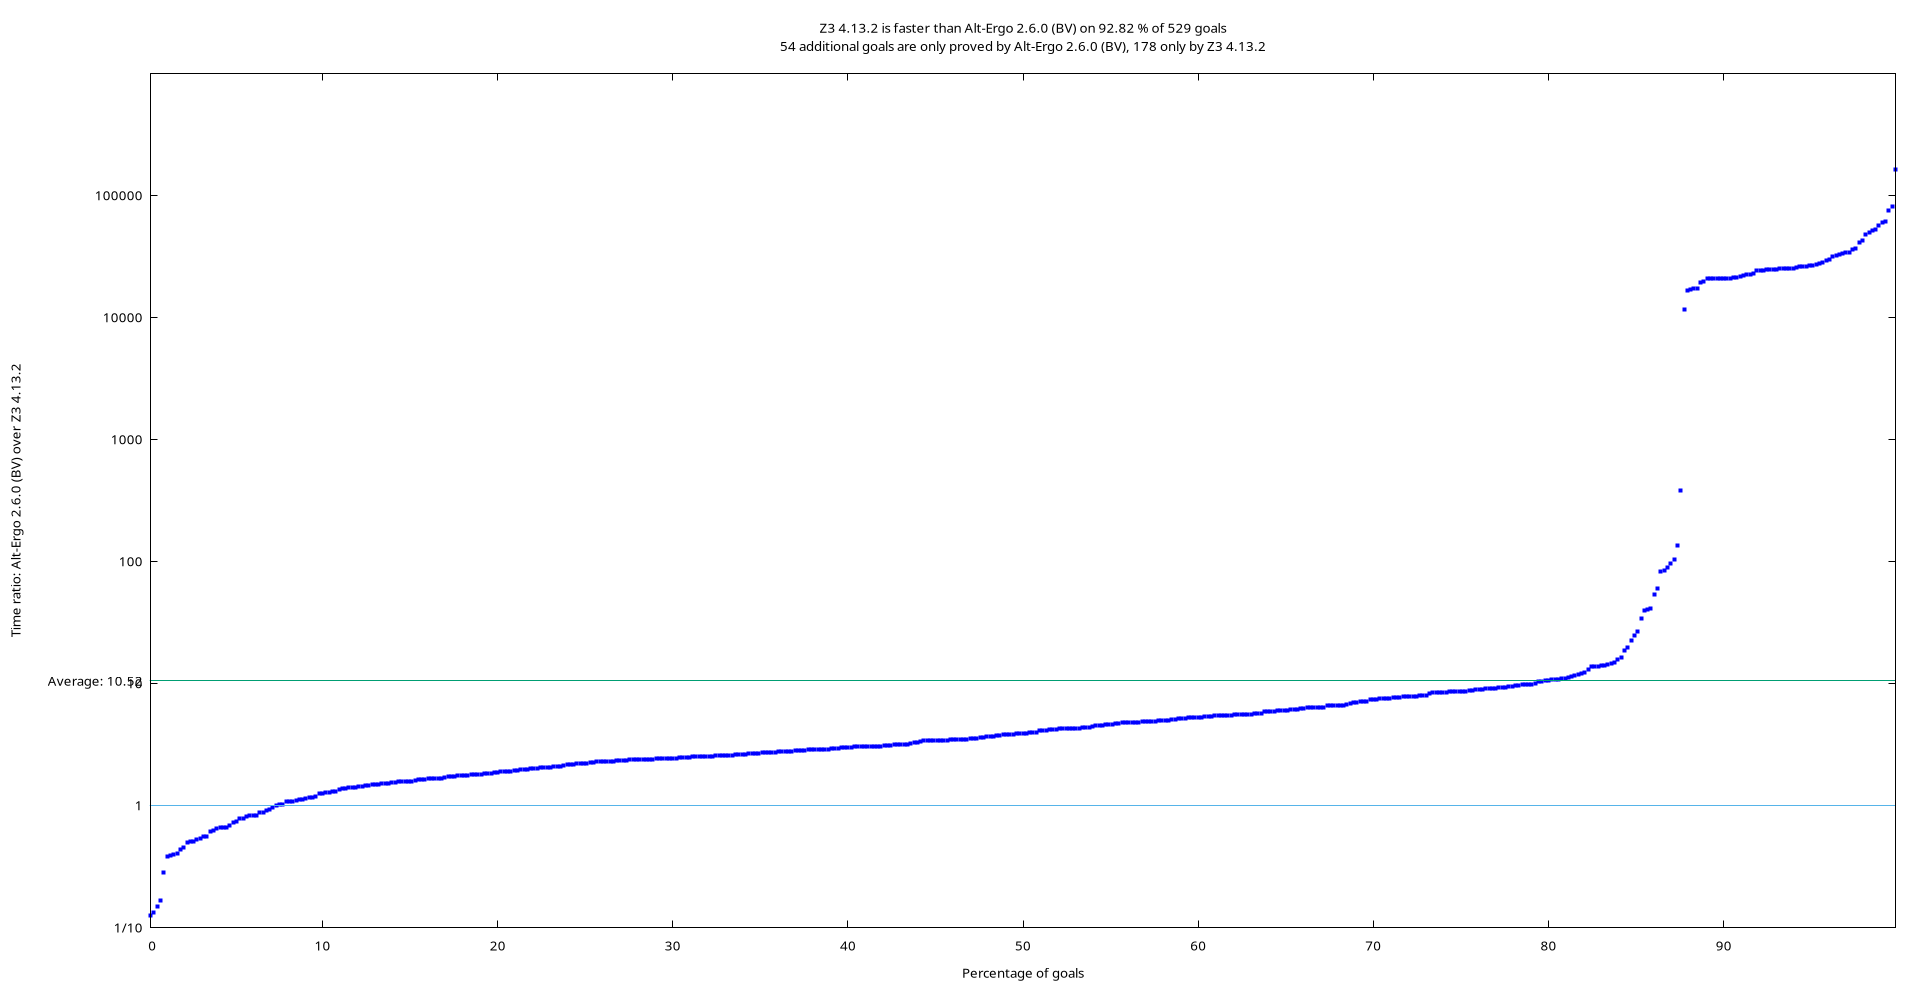
\includegraphics[width=\textwidth]{Z3vsAEBV.png}

\end{frame}

\begin{frame}{Actions regarding bitvectors}

  What else?

  \begin{itemize}
  \item Put a specific set of benchmarks in the Decysif git?
  \item Test with J3?
  \item OCamlPro: add support for \texttt{bv2int}?
  \item Side remark: could AE support non-standard \texttt{pow2} function (cvc5 has \texttt{int.pow2})
  \item ?
  \end{itemize}

\end{frame}

\subsection{Polymorphism, ADTs}

\begin{frame}{Polymorphism}

  Issue to report regarding counterexamples

\end{frame}

\begin{frame}{ADTs}

  AE 2.5.4 support for ADTs was not satisfactory enough

  AE 2.6.0 to be tested ?

  Should we design a set of benchmarks dedicated to ADTs?

\end{frame}

\subsection{Steps}

\begin{frame}{About ``Steps''}

  \begin{itemize}
  \item Uncaught exception (issue
    \url{https://github.com/OCamlPro/alt-ergo/issues/1244}). Also:
    \begin{itemize}
    \item should be a ``per-query'' limit
    \item same for time limit indeed: is there a per-query time limit in AE?

      seems there is: \texttt{-{}-timelimit-per-goal}
    \end{itemize}
  \item Steps that do not advance enough?
    \begin{itemize}
    \item Not easy to reproduce... might be related to the need of
      per-query limits for time steps
    \end{itemize}
  \end{itemize}

\end{frame}

\begin{frame}{Actions regarding ``steps''}

  \begin{itemize}
  \item{} [OCamlPro] Implement a \texttt{-{}-steps-per-goal} option?
  \item{} [OCamlPro] Make sure steps ``advance'' enough in any part of the code
  \end{itemize}

\end{frame}

\subsection{Benchmarks Decysif}

\begin{frame}{Benchmarks Decysif}

  \begin{itemize}
  \item Number of VCs and number of SMT files not coherent? (issue reported by Basile)
  \item Others?
  \end{itemize}

\end{frame}

\section{Rust}

\begin{frame}{Rust and Creusot}

  \begin{itemize}
  \item Is OCamlPro ready to start a Rust project using Creusot?
  \item\relax [long-term] discussion about ``industrialization'' of Creusot
  \end{itemize}

\end{frame}


\end{document}



%%% Local Variables:
%%% mode: latex
%%% TeX-master: t
%%% TeX-PDF-mode: t
%%% mode: flyspell
%%% mode: accents
%%% ispell-local-dictionary: "british"
%%% End:
